% ============================================================================
%  GENERAL PORTFOLIO -- hardware and software together
%  See also:
%    Mohammed Aljomaily Hardware Portfolio.tex
%    Mohammed Aljomaily Software Portfolio.tex
%    Mohammed Aljomaily Baykar Portfolio.tex   (hardware-led, for Baykar)
%
%  Build from inside portfolio/ so the img/ paths resolve:
%      pdflatex "Mohammed Aljomaily General Portfolio.tex"
% ============================================================================

\documentclass[11pt,a4paper]{article}

\usepackage[T1]{fontenc}
\usepackage{lmodern}
\usepackage[margin=1.9cm]{geometry}
\usepackage{enumitem}
\usepackage{graphicx}
\usepackage[hidelinks]{hyperref}

% Float placement tuning: prefer figures on pages that also carry text, and
% only build a dedicated figure page when it would be almost completely full.
\renewcommand{\topfraction}{0.92}
\renewcommand{\bottomfraction}{0.92}
\renewcommand{\textfraction}{0.06}
\renewcommand{\floatpagefraction}{0.9}

\setlength{\parindent}{2pt}
\setlength{\parskip}{5pt}
\pagestyle{empty}
\hyphenpenalty=1200
\exhyphenpenalty=1200
\emergencystretch=1.5em

\newcommand{\entry}[2]{%
  \vspace{6pt}%
  {\Large\bfseries #1}\hfill{\itshape\small #2}\par
  \vspace{3pt}\hrule\vspace{4pt}%
}

\newcommand{\domain}[1]{%
  \vspace{16pt}%
  {\LARGE\bfseries #1}\par
  \vspace{3pt}\hrule\vspace{8pt}%
}

\begin{document}

\begin{center}
    {\LARGE \textbf{Mohammed Aljomaily}}\\[3pt]
    {\large Portfolio}\\[6pt]
    {\small Computer Engineering Student \textbar{} Embedded Systems, PCB Design \& RF \textbar{} Backend \& Applied AI}\\[3pt]
    {\small Beylikd\"uz\"u, Istanbul, Turkey \textbar{} +90 535 273 6199 \textbar{}
    \href{mailto:mohammedaljomaily06@gmail.com}{mohammedaljomaily06@gmail.com}}\\[2pt]
    {\small \href{https://v01d.dev}{v01d.dev} \textbar{} \href{https://github.com/V01Ddev}{github.com/V01Ddev}}
\end{center}

\entry{Preface}{}

I am a Computer Engineering student at Istanbul Ayd{\i}n University. This
document is a record of what I have designed, built and shipped, across hardware
and software.

I came into engineering through software, somewhat by accident. During a gap
year I took an internship at Applab in Doha, and it turned into fourteen months
of production work for enterprise clients: backend services for an AI video
platform used by Al Jazeera, and an AI chatbot for the General Authority of
Customs. It was serious work and I am proud of it. But the thing I actually did
with my own time was different. I was designing circuit boards, etching them at
my kitchen table, soldering them, and flying what I had built.

The two halves feed each other. Writing software taught me what production
actually demands, which is why I build retry handling and state logging into a
media pipeline rather than treating them as afterthoughts. Building hardware
taught me that the abstraction eventually ends and something physical has to
work, which is why I care about what happens at the layer below.

Almost everything in the hardware section was made at a desk at home, including
the circuit boards themselves. Where a project is unfinished or was not
continued, I have said so.

% ===========================================================================
\domain{Hardware}
% ===========================================================================

\entry{5-Inch FPV Quadcopter}{2026}

A complete 5-inch FPV aircraft, built from parts and configured from scratch:
\textbf{Mario 5} frame, \textbf{Mamba MK4 F722} flight controller, \textbf{F40 V2}
motors, and \textbf{DJI O4 Lite} video on \textbf{6S}. I configured Betaflight,
set up the \textbf{ExpressLRS 2.4\,GHz} control link between a RadioMaster Pocket
running EdgeTX and the receiver, and tuned the aircraft to fly the way I wanted
it to rather than the way it arrived.

I wrote the preflight checklist for this aircraft myself, as a ground-check
procedure I run before every session. It is not a formality: on a machine with
propellers, batteries and a radio link, the failures that hurt are the boring
ones.

Alongside the airframe I built out the rest of the workflow, including GyroFlow
stabilisation for footage from a GoPro HERO7 with ND filters, and a custom EdgeTX
sound pack and 3D-printed stick ends for the radio.

\begin{figure}[!htbp]
\centering
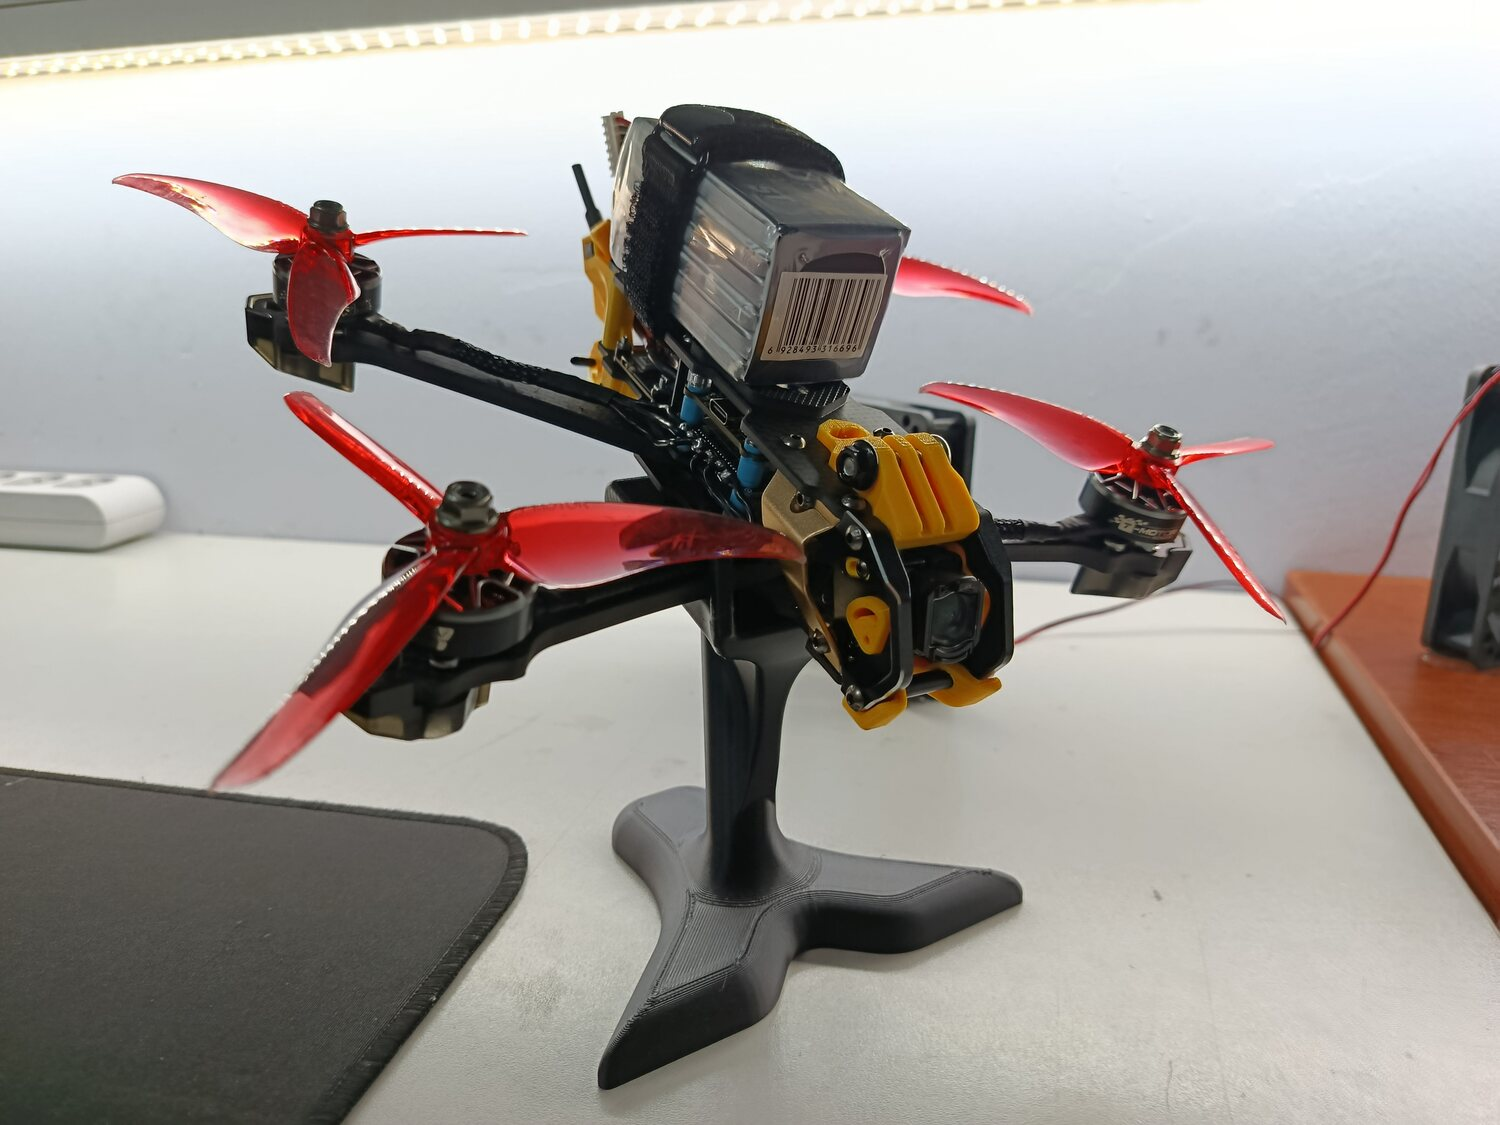
\includegraphics[width=0.38\textwidth]{img/drone.jpg}
\caption{The finished 5-inch build.}
\end{figure}

\entry{Dual-Transceiver ESP32 Jammer Board}{2026}

A two-layer ESP32 jammer board I designed in \textbf{KiCad} for educational study
of 2.4\,GHz protocols, and then fabricated by hand at home: an \textbf{ESP32
DevKit V1} carrying \textbf{two nRF24L01+PA+LNA} transceivers, each on its own
SPI bus (HSPI and VSPI) so both radios operate independently, plus an SSD1306
OLED for status and an optional TP4056 charging circuit for a Li-Ion cell. The
finished board is 64.14 $\times$ 77.47\,mm.

I did not use a fabrication house. Shipping to Turkey plus the cost of a local
service made no sense for boards this size, so I generate the artwork, transfer
it, etch it, drill it and assemble it myself. That decision shaped the design:
the first layout was two layers and turned out to be close to impossible to
produce by hand, so I enlarged the vias, reworked the routing for the process,
cleared every DRC error, and made it a second time. The second board works.

The firmware is adapted from an existing open-source project rather than written
from scratch. I wanted my hardware to be fully compatible with it, so the
engineering work on my side was the board, the schematic capture, the custom
footprints and the fabrication.

\begin{figure}[!htbp]
\centering
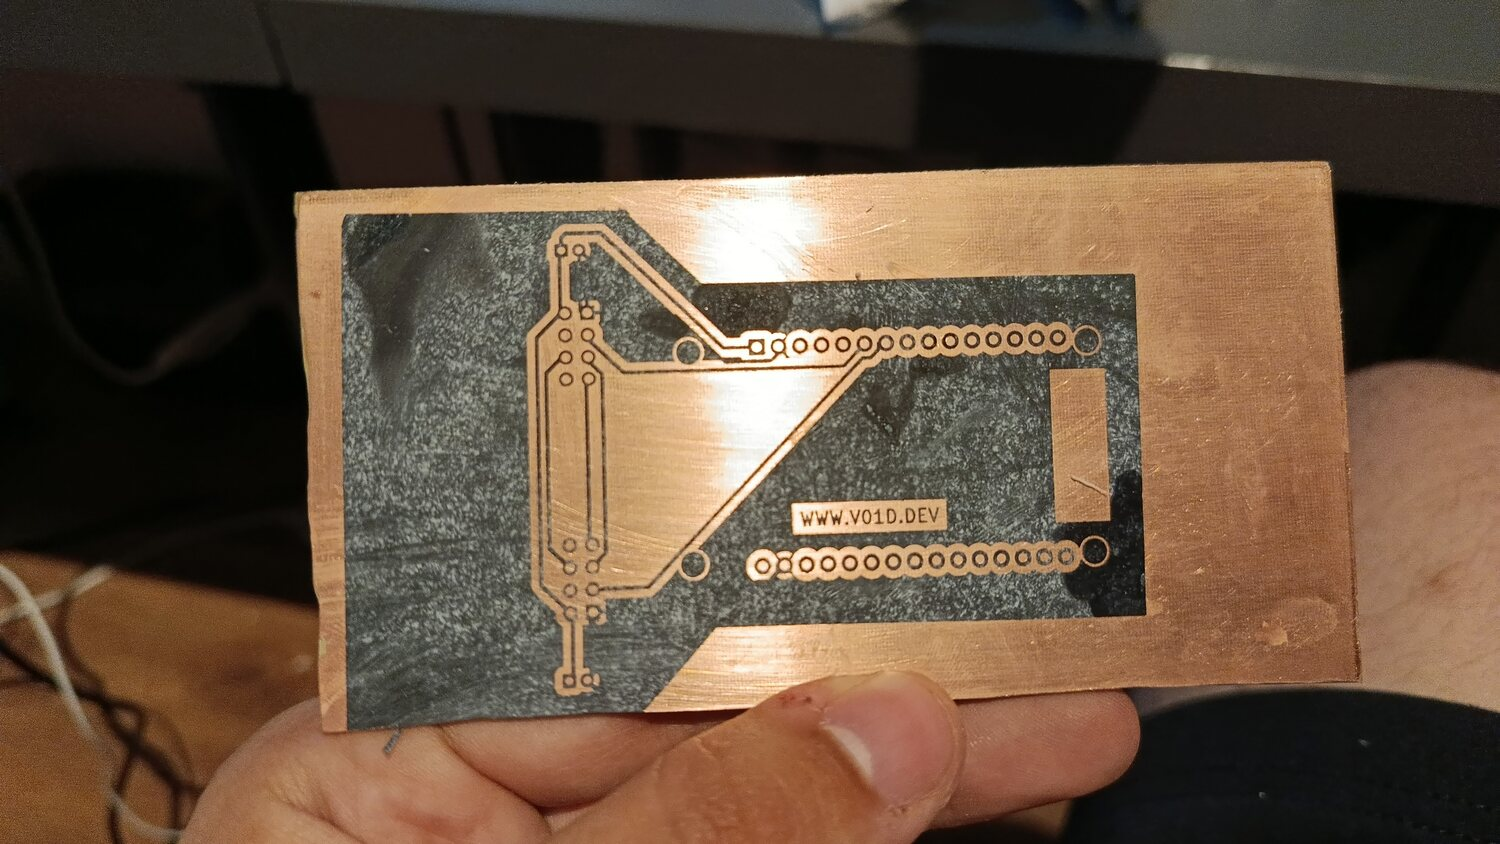
\includegraphics[width=0.35\textwidth]{img/rf-transfer.jpg}
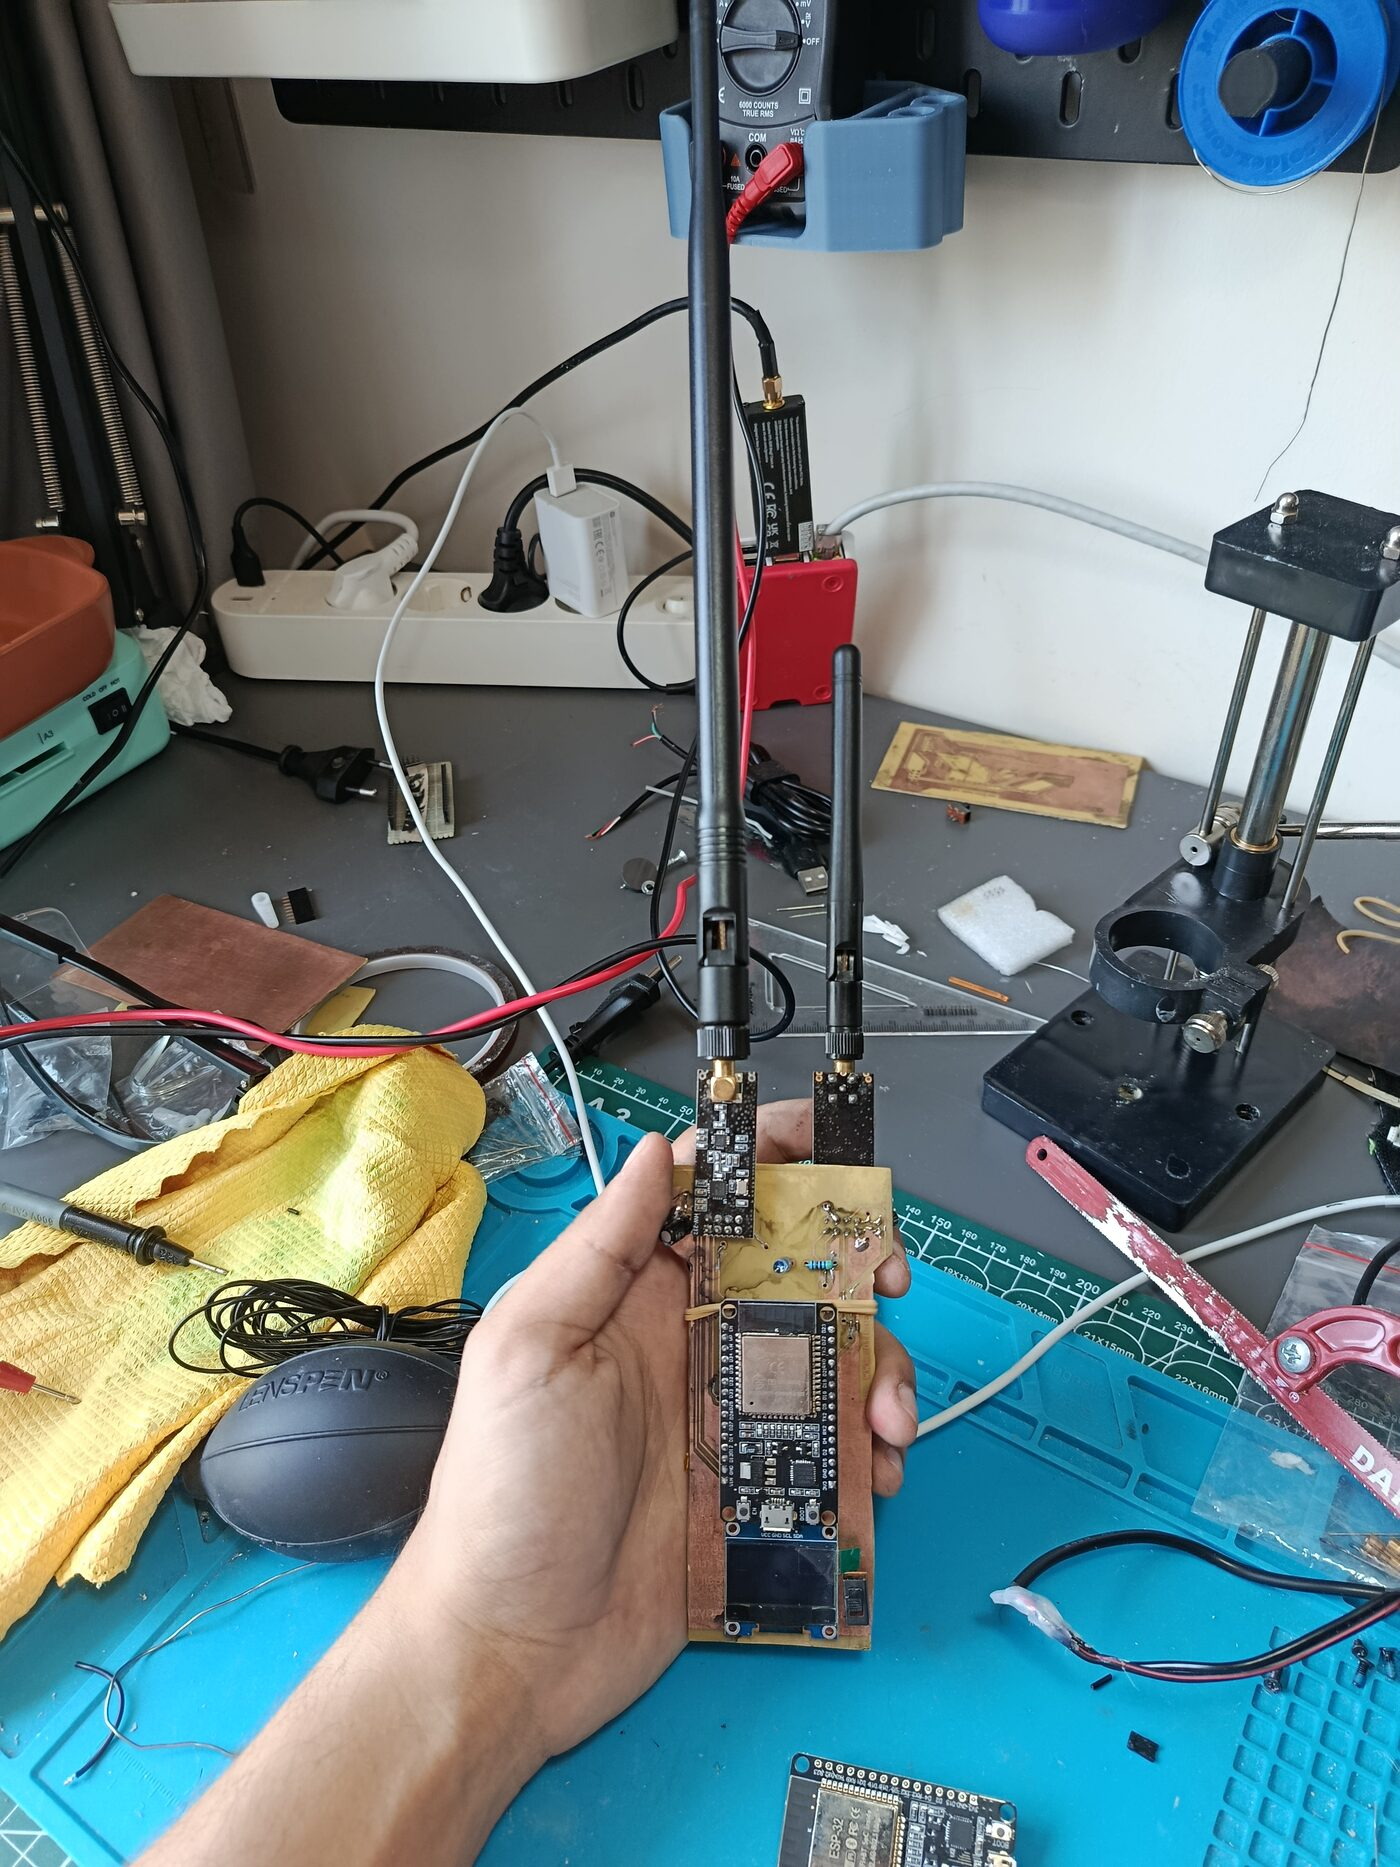
\includegraphics[width=0.25\textwidth]{img/rf-board.jpg}\hspace{1.5em}%
\caption{The first revision: toner transferred onto copper, and the same board assembled.}
\end{figure}

\begin{figure}[!htbp]
\centering
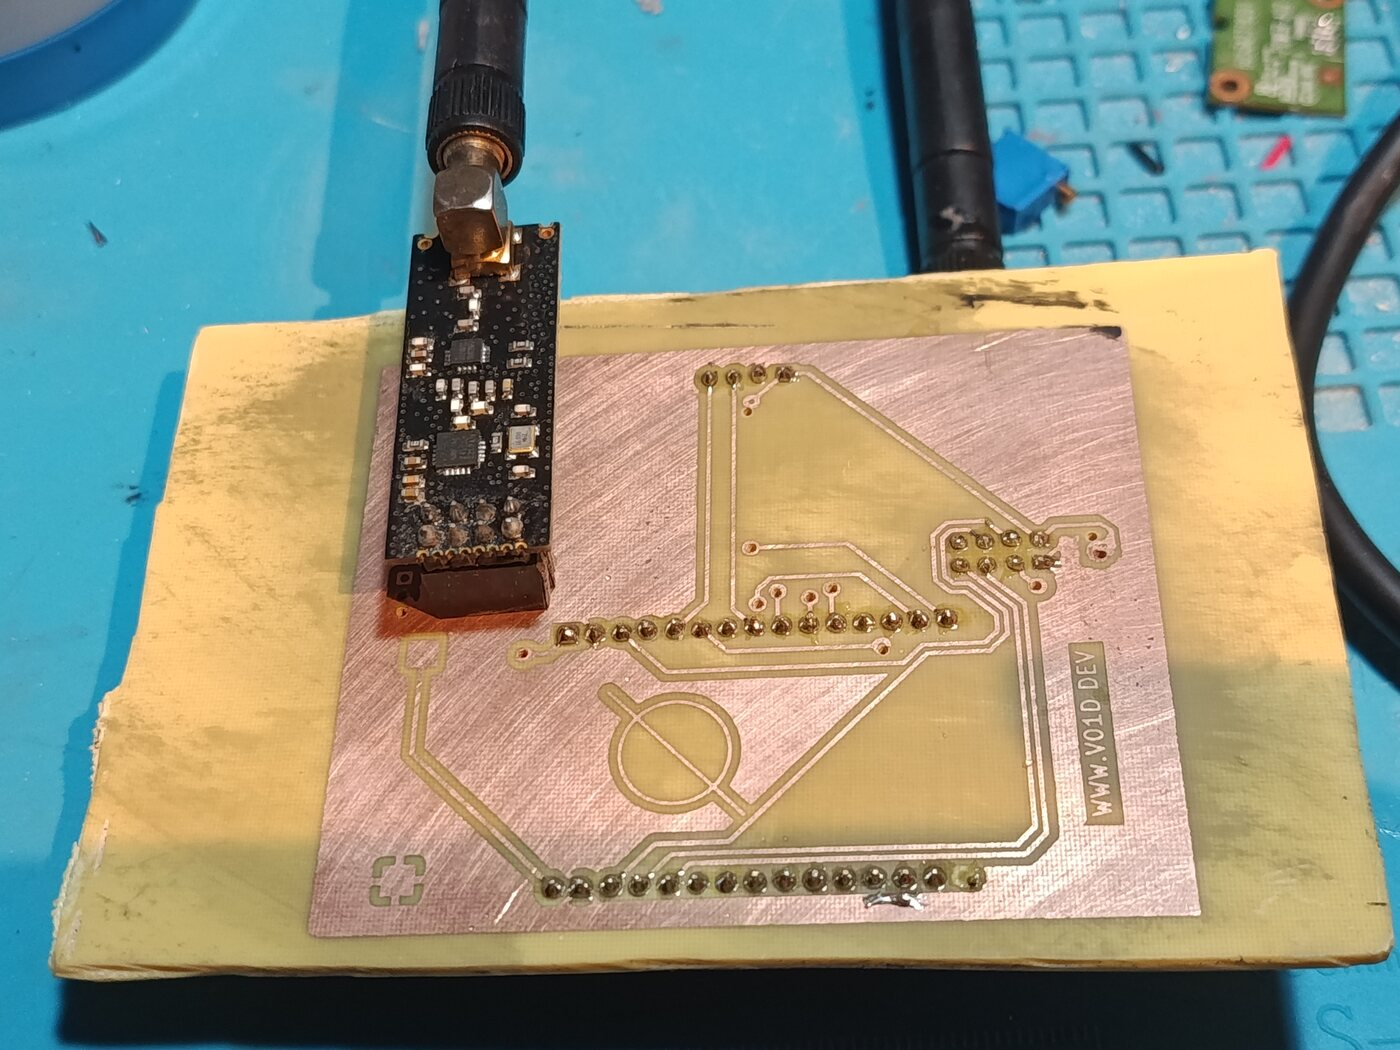
\includegraphics[width=0.31\textwidth]{img/rf-etched.jpg}\hspace{1em}%
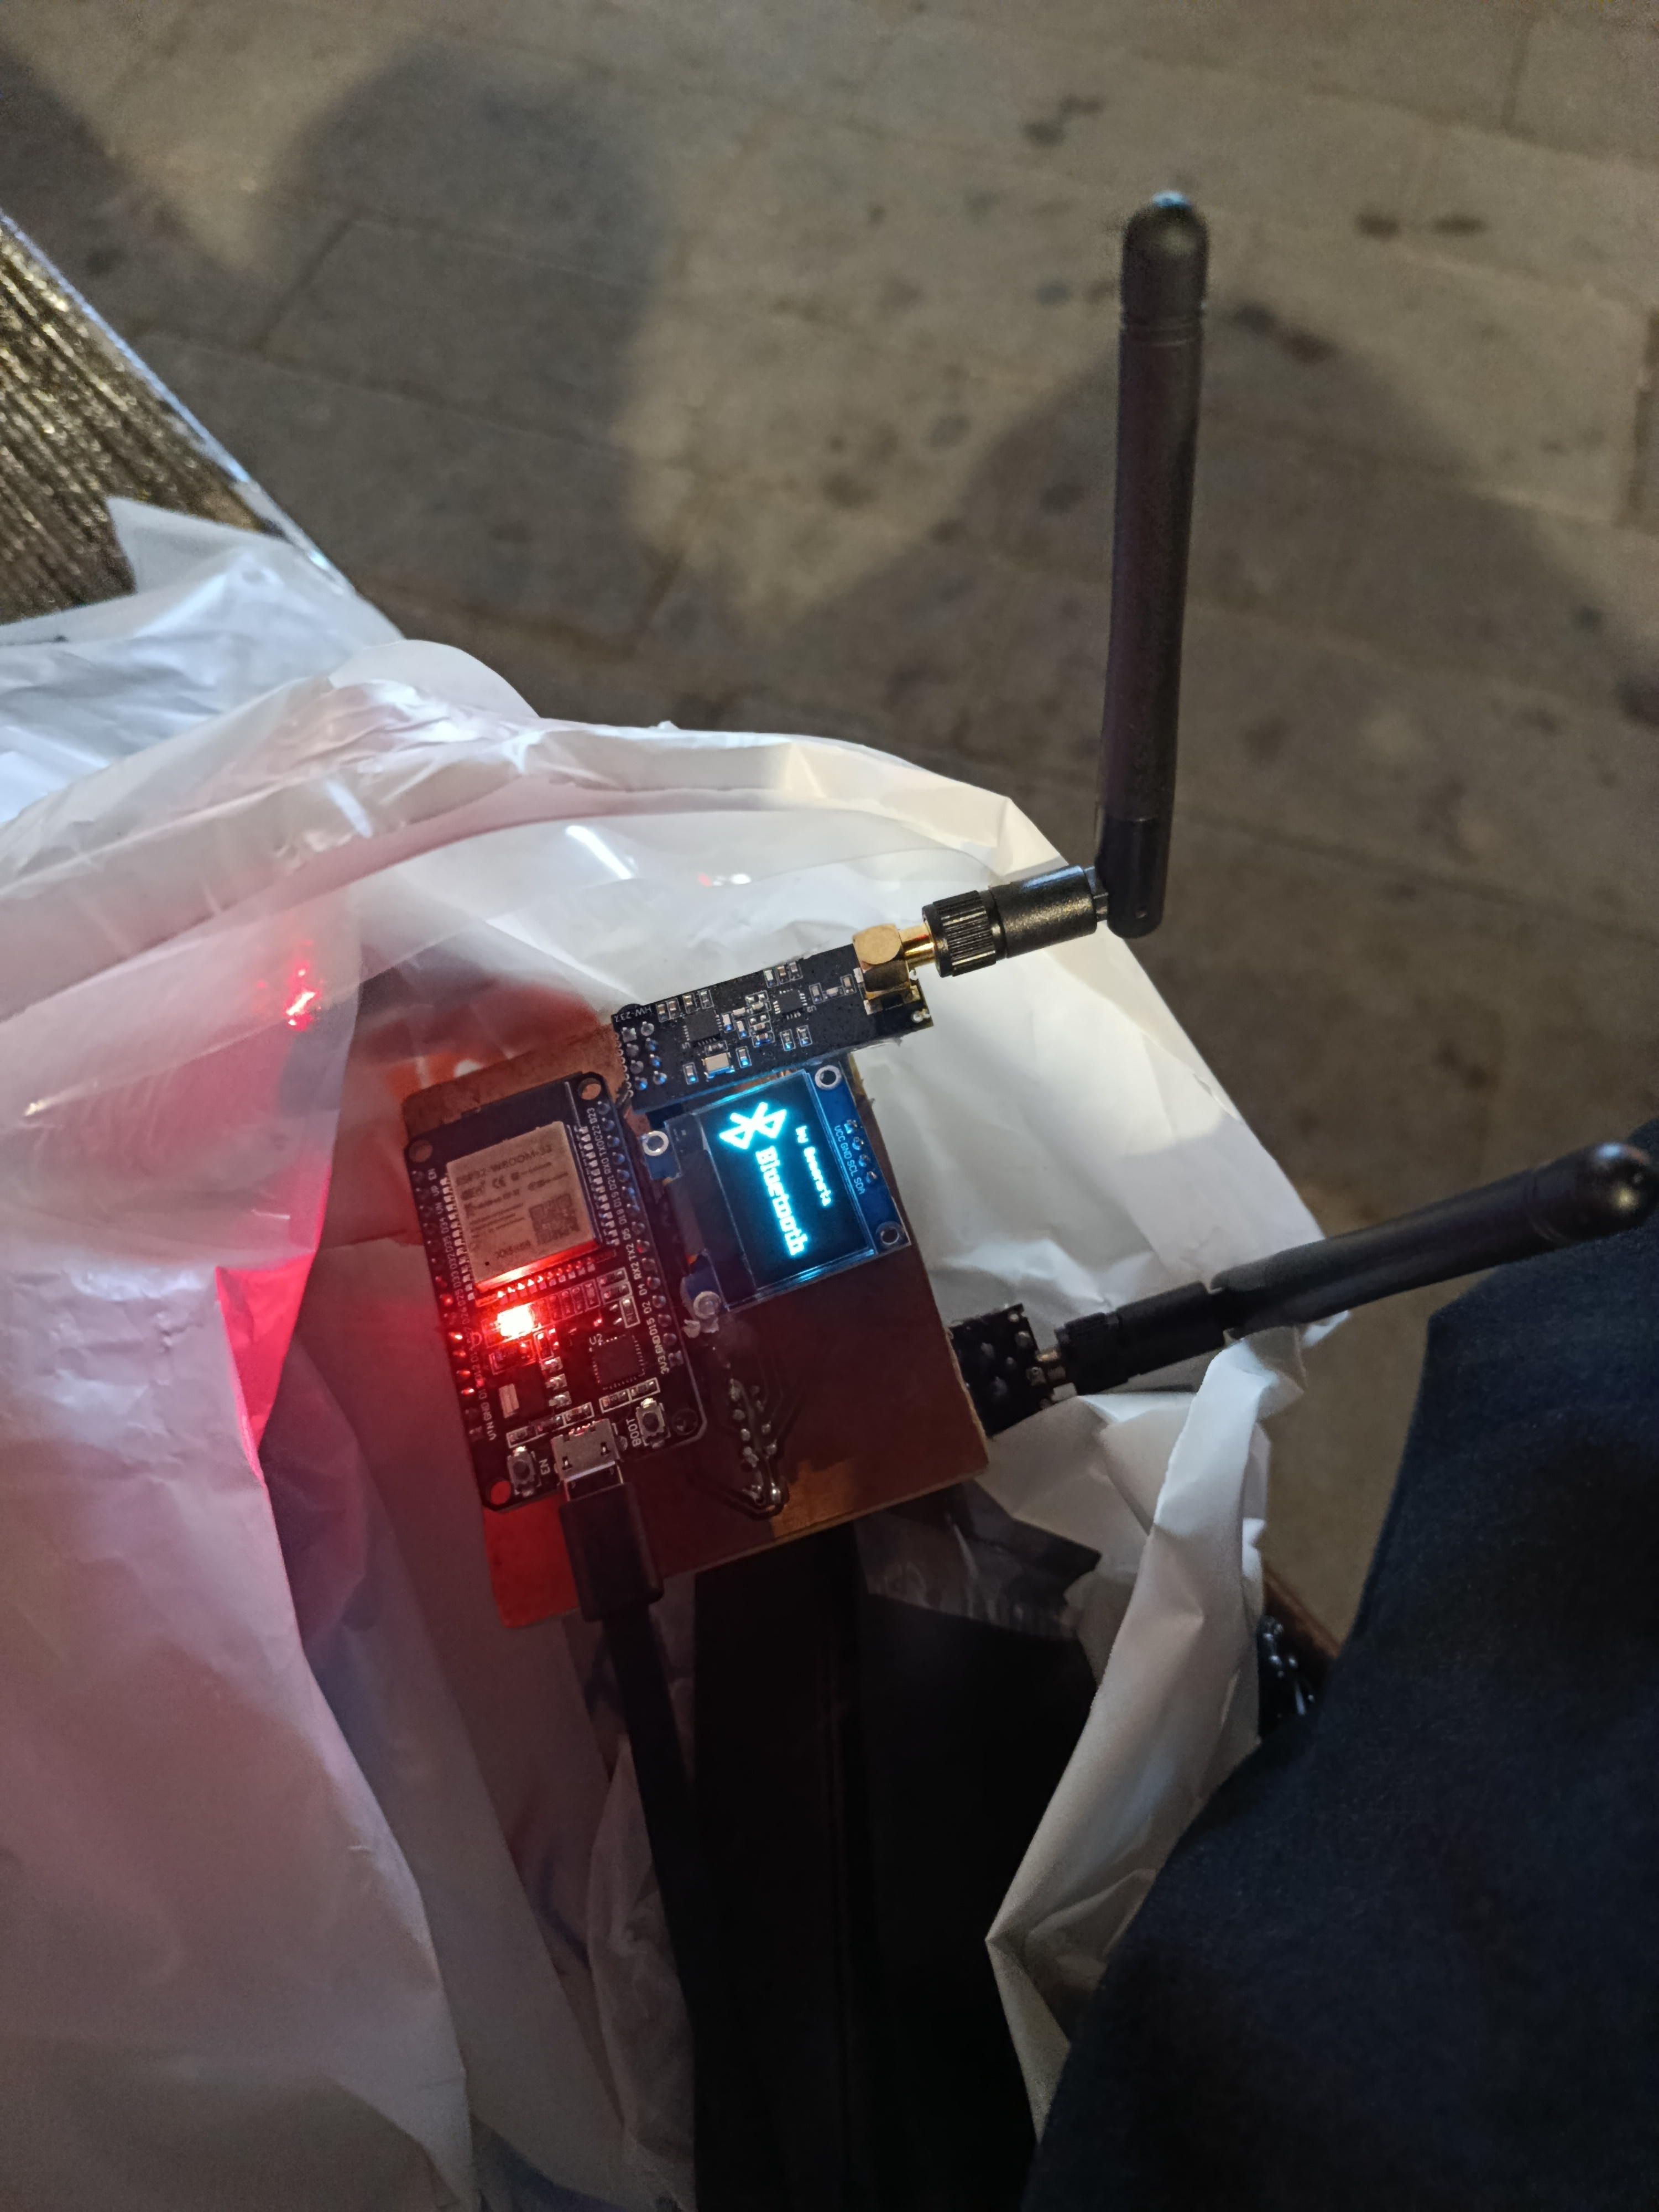
\includegraphics[width=0.31\textwidth]{img/rf-final.jpg}
\caption{The final revision after etching, and the finished board in use.}
\end{figure}

\begin{figure}[!htbp]
\centering
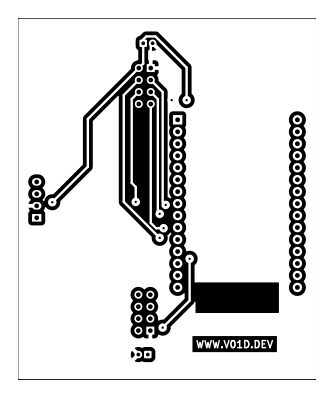
\includegraphics[width=0.17\textwidth]{img/rf-fcu.png}\hspace{2.5em}%
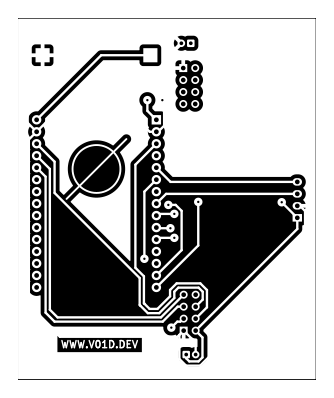
\includegraphics[width=0.17\textwidth]{img/rf-bcu.png}
\caption{Front and back copper layers exported from KiCad. These are the etch artwork.}
\end{figure}

\entry{Flight Telemetry \& Attitude Indicator}{2026}

An ESP32 telemetry system for small aircraft, pairing an \textbf{MS5611}
barometer with an \textbf{MPU6050} inertial measurement unit. I fused the two
sensors through a complementary filter (to correct the gyroscope's drift against
the accelerometer's noise) and streamed attitude and altitude over serial at
roughly 50\,Hz.

The ground station is written in Python with \textbf{PySide6} and \textbf{Qt QML},
drawing a live artificial horizon from the incoming telemetry. I started it in
Pygame and migrated it to QML partway through, because the original approach
could not render smoothly enough to be useful as an instrument.

\begin{figure}[!htbp]
\centering
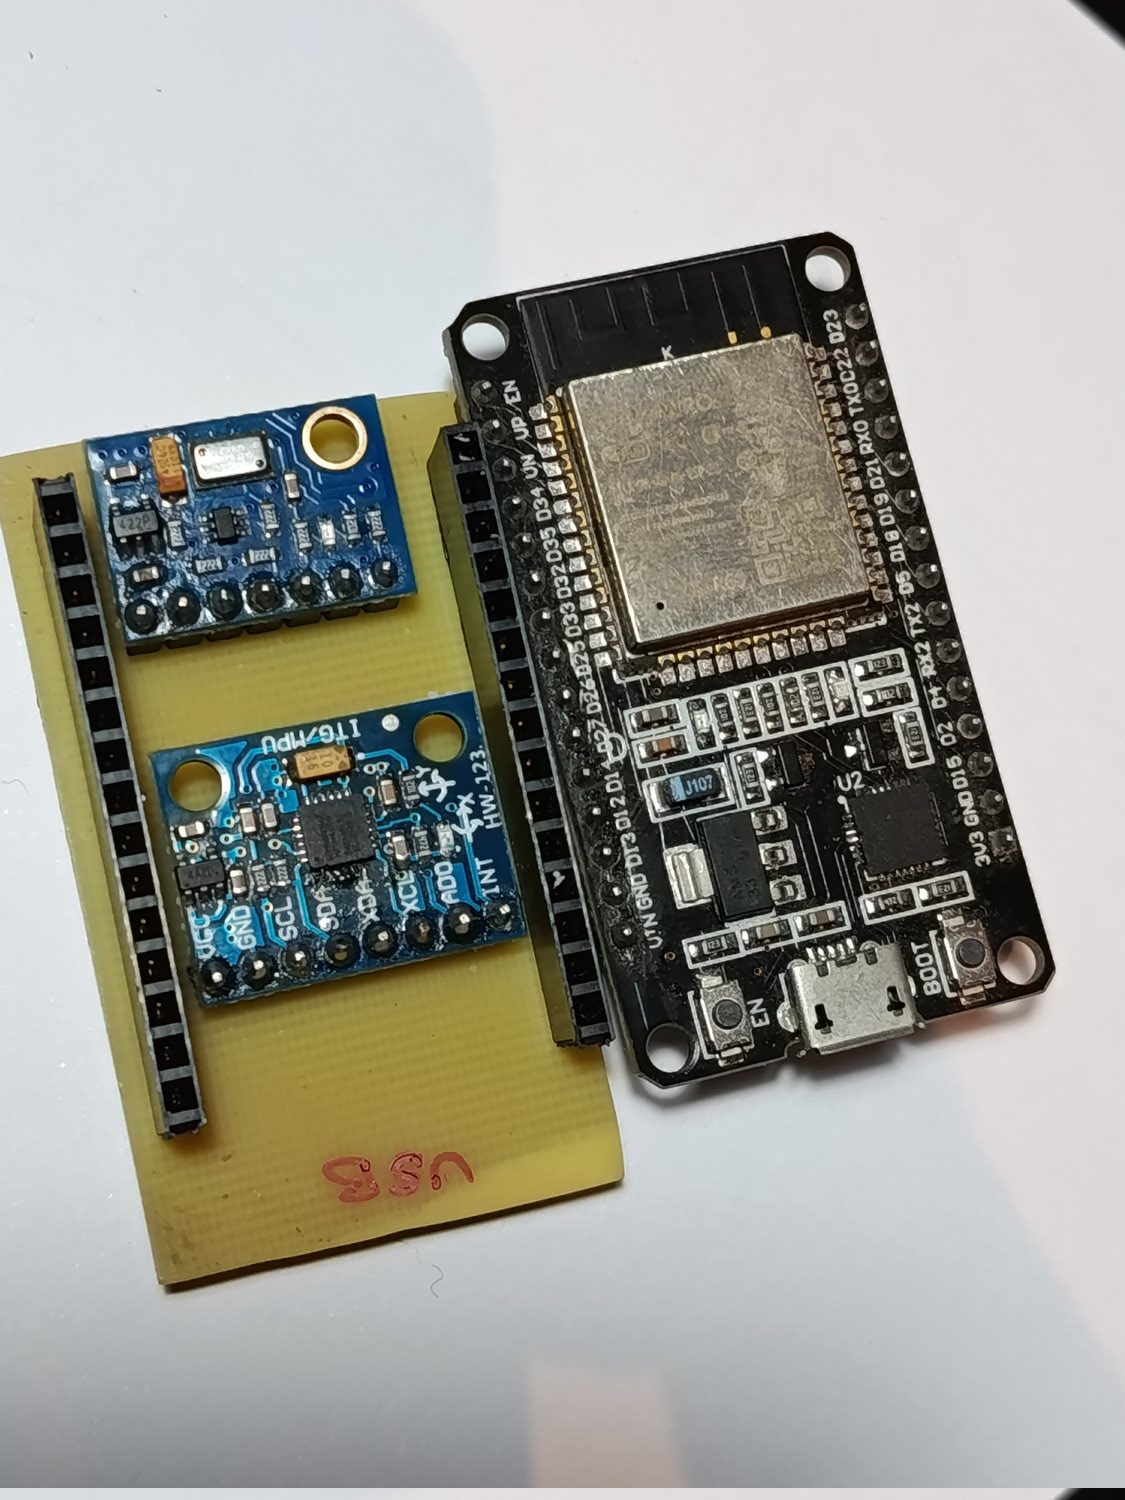
\includegraphics[width=0.30\textwidth]{img/telemetry.jpg}
\caption{The telemetry board.}
\end{figure}

\entry{Discrete Transistor Logic Gates}{2026}

A board that implements \textbf{AND, NOT, OR and NAND} gates from individual
transistors, with no logic ICs anywhere: seven \textbf{PN2222A} NPN transistors
in resistor--transistor logic, with LEDs as outputs and tactile switches as
inputs.

I built this to work below the abstraction layer. It is easy to use a 74-series
chip and never think about what is inside it. Designing the same gates from
transistors means reasoning about base current, saturation and voltage levels
directly. I designed the schematic, routed the two-layer board with a ground
plane, and fabricated the first revision. It is currently under debug, and I am
working through the fault.

\begin{figure}[!htbp]
\centering
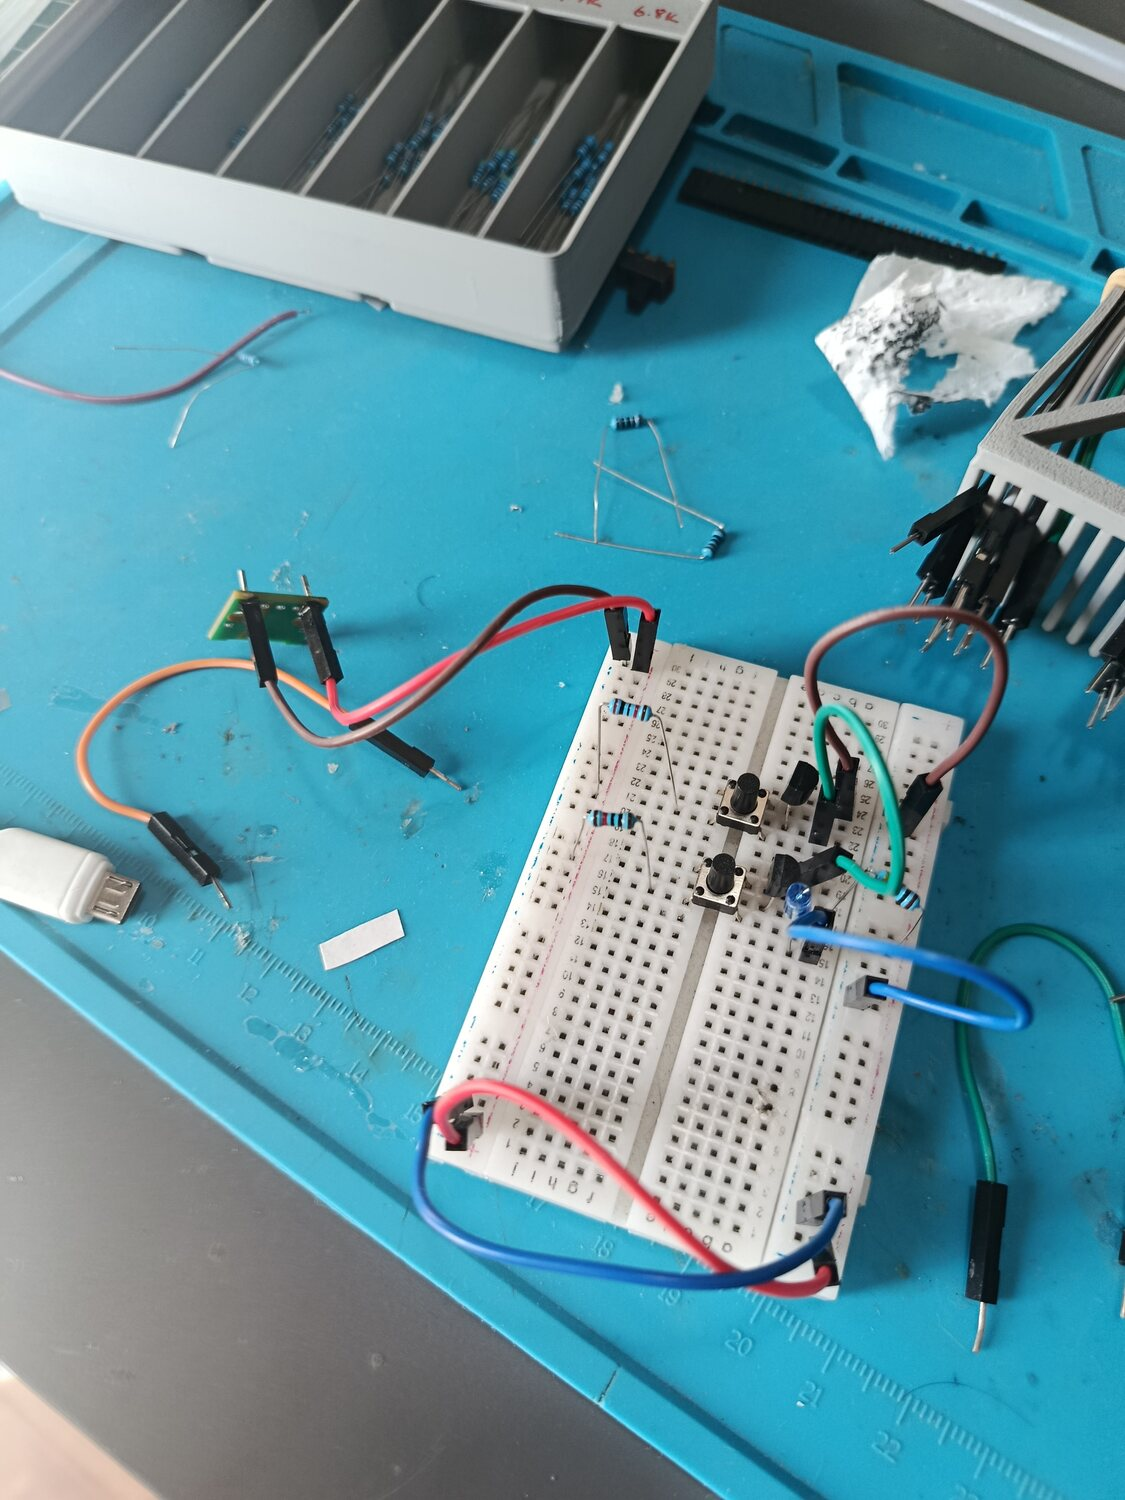
\includegraphics[width=0.38\textwidth]{img/logic-gates.jpg}
\caption{The gate circuits on a breadboard, before committing to the PCB.}
\end{figure}

\entry{RC Aircraft \& Radio Link}{2025--2026}

Two fixed-wing designs, drawn and built from first principles rather than from a
kit. \textbf{FCF-1} uses a 9\,mm carbon fibre main spar with a \textbf{NACA 63412}
airfoil, and I modelled the airframe in \textbf{FreeCAD}: wing structure, servo
mounts, pushrods, control horns, aileron hinges and motor mount, all as parts
that could actually be cut and printed. It has flown. A later design,
\textbf{Simple-Glider}, was built to be easy to reproduce from foam board and
printed parts, with a full build guide covering dimensions and part counts.

For the radio link on these aircraft I wrote the transmitter and receiver
firmware myself: four analog channels encoded over \textbf{ESP-NOW} at 20\,Hz,
driving servos on the receiving end, with a failsafe that recentres every channel
if the link is lost for three seconds.

\entry{Published KiCad Library}{2026}

The SSD1306 0.96-inch OLED module is one of the most common parts in hobby
electronics, and I could not find a KiCad symbol and footprint for it that
worked in a current version of KiCad. So I made one and published it: a native
\textbf{KiCad 9} symbol and footprint, converted from an earlier library with
the original \textbf{CC BY-NC-SA} attribution preserved as its licence requires.
It is not a file sitting in a drawer; I use this footprint in my own boards.

\entry{Home PCB Fabrication}{ongoing}

Everything with a circuit board in this portfolio was made by hand, and the
process itself has been a project. I generate artwork from KiCad, transfer it to
copper, etch, drill and assemble, and I designed for that process on the boards
above. I modelled a \textbf{toner transfer tool} in FreeCAD specifically for
this workflow, and I write up the method on my site because the information that
helped me most came from other people doing the same thing.

I also model and print mechanical parts, from enclosures for the boards above to
a reversible USB power modification for a FlySky i6X transmitter that fits into
the battery compartment without altering the case.

\entry{Router Firmware Reverse Engineering}{2026}

I took a Xiaomi router apart to understand how it boots. I located the UART
header on the board and connected to it to capture the boot log, which is the
most direct way to see what a device does before any of its own software takes
over. The console turned out to be locked, so I moved to the flash instead and
extracted the firmware image, which showed the firmware was built on an
open-source base. I stopped there when the university term started.

\begin{figure}[!htbp]
\centering
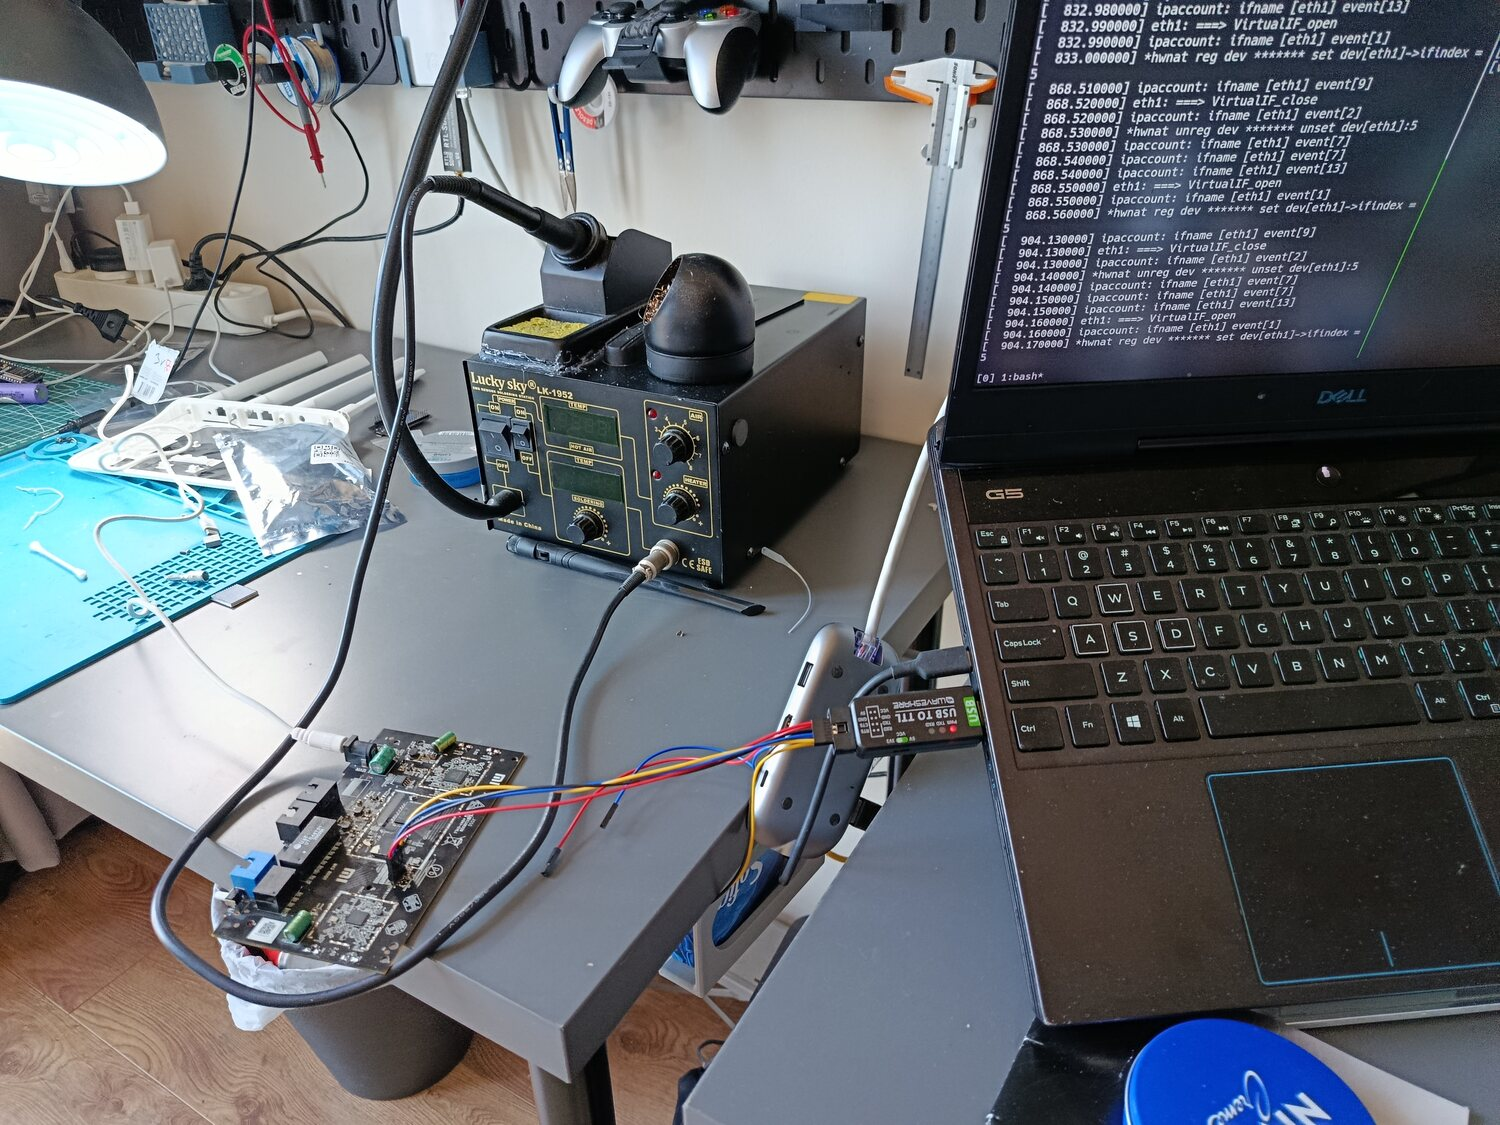
\includegraphics[width=0.40\textwidth]{img/router-uart.jpg}
\caption{Capturing the boot log over UART.}
\end{figure}

% ===========================================================================
\domain{Software}
% ===========================================================================

\entry{Al Jazeera: AI Video Platform}{2025--2026}

My main body of work at \textbf{Applab}, and by some distance the largest system
I have worked on. The platform takes an uploaded video, strips silence and
filler words, re-transcribes it, and produces a translated video with subtitles.
I was the primary author of the backend: the API service, the asynchronous job
worker, and the projects API.

\textbf{Architecture.} An event-driven pipeline on \textbf{Azure Container Apps}.
A \textbf{Quart} API running under Hypercorn writes a state document to
\textbf{Cosmos DB} and pushes a message onto \textbf{Azure Storage Queues}. A
second, ingress-disabled container polls the queue and dispatches the work, then
writes status back to Cosmos. The two services scale on different signals: the
API on concurrent HTTP requests, the worker on queue depth.

\textbf{Media and AI.} I integrated \textbf{Azure Cognitive Services Speech}
using the fast transcription endpoint, and the Video Translation API, which I
migrated to a newer API version. Transcription covers \textbf{14 locales}, with
automatic fallback to \textbf{Azure OpenAI Whisper} for anything outside that
set. Translation and analysis run against \textbf{GPT-4o}.

\textbf{The hard parts.} Long-running media work fails in ways that are not
obvious. I built poison-message routing so a job that will never succeed stops
blocking the queue, a bounded retry loop with backoff around the translation
lifecycle, and per-action state logging so a stuck job can be traced. I also
wrote the subtitle alignment logic, including WebVTT handling that uses
half-open interval arithmetic so adjacent cues which merely touch at a boundary
do not get merged into one.

\entry{General Authority of Customs: AI Chatbot}{2025--2026}

An enterprise AI chatbot built from scratch for a government client, on
\textbf{FastAPI} and \textbf{Semantic Kernel}. Retrieval runs through
\textbf{Azure AI Search} with vector search for semantic document lookup rather
than keyword matching, and I wrote the conversation history layer myself rather
than taking it from a framework, which meant owning how context is trimmed and
carried between turns.

\entry{Invest Qatar: Document Generation}{2026}

A backend that turns AI-generated structured JSON into formatted \textbf{DOCX}
documents. The team's assumption was that this needed an external service; I
built it in-process with Python file I/O instead, at roughly \textbf{30\,ms per
document}, which removed a network dependency and a per-document cost from the
pipeline.

\entry{University RAG Chatbot}{2025}

A retrieval-augmented chatbot answering questions over Istanbul Ayd{\i}n
University's documentation. \textbf{LangChain} with OpenAI embeddings and
\textbf{MongoDB Atlas Vector Search} for retrieval, and a companion
\textbf{Selenium} scraper that walked the university site and extracted
\textbf{184 documents} from a 200-entry sitemap.

The part I would point at is the ingest pipeline. Rather than rebuilding the
index on every run, it content-hashes each page and diffs against what is
already stored, so only pages that actually changed are inserted, updated or
deleted. The site changes constantly and most of it does not change at all; this
makes re-ingesting cheap instead of an event.

\entry{TIPOT: PDF Organising Tool}{2024--2026}

A web application for reordering and merging PDF pages, built with
\textbf{Flask} and \textbf{PyMuPDF} and shipped as a Docker image with a
compose file. It is the project I am most glad I put online: an outside
contributor found it, used it, and submitted a pull request that I reviewed and
merged. Maintaining something other people depend on, and integrating someone
else's work into it, taught me more than the code did.

\entry{Aircraft Engine Trend Analysis}{2026}

Analysis of multi-model turbine engine trend data for the 747, 767, 777 and 787
in Python. I worked through exhaust gas temperature, fuel flow, and N1 and N2
vibration signatures, comparing behaviour across the fleet and over time, and
wrote up what the correlations suggested about wear, sensor bias and thermal
drift.

\entry{Smaller Projects}{}

\begin{itemize}
    \item \textbf{v01d.dev} --- Personal site and technical blog, hand-built with Hugo and maintained since 2021, including write-ups of hardware work.
    \item \textbf{deltastack.dev} --- Landing site for a student engineering team; Next.js, React and Tailwind. Sole author.
    \item \textbf{table2csv} --- Converts the university course-schedule site into printable and Google Calendar CSV, with a manual-paste fallback for pages that block automation.
    \item \textbf{LAN Scanner} --- Threaded network ping sweep, implemented in both C++ and Python.
\end{itemize}

\vspace{8pt}
\hrule
\vspace{6pt}

\textbf{Toolchain.} C and C++ on ESP32 and ESP8266; Python, Go, TypeScript.
KiCad 9/10 for schematic capture and PCB layout, FreeCAD for mechanical design,
FDM printing. SPI, I\textsuperscript{2}C, UART, PWM and ADC at the hardware
level; nRF24L01, ESP-NOW, ExpressLRS, Bluetooth and IR for radio. On the
software side: Azure Container Apps, Cosmos DB, Blob and Queue Storage,
Cognitive Services, Azure OpenAI and AI Search; FastAPI, Quart, Semantic Kernel,
LangChain; Docker, Linux, Postgres, MongoDB, pandas.

\end{document}
